\section*{A-5. Deep Neural Network (DNN)}

\subsection*{a. Unveil the power of deepness}

The basic observation suggests that the error rate of testing dataset (or unseen samples) with deep neural network is much smaller than the one of the "fat" neural network, although they may have the same neurons. So to avoid overfitting, we often implement neural network architecture as deep layers.

However, the most important reason that a DNN can outperform a "fat" ANN is the fact that most of object, data in real world has complex hierachy. The deep nets have the ability to build up these complex hierachy of concepts.

A "fat" ANN need to answer the complicated question at once. Although basically that can be done as proved by Universality theorem, the performance or learning speed is really bad. On the other hand, a DNN can decompose any complicated problems into smaller ones, which are often easier, until these questions are so trivial that DNN can answer with just a single neuron. This is the same as the way human (brain) solve any problem in real life: divide and conquer. This can be seen clearly in the case of visual recognition tasks.

Suppose we need to build a ANN that answer if a given image contains a human face. To make problem easier, we can build the sub-network that answer basic questions.  And of course, these questions can even be divided smaller until the neurons work with individual pixels. In other word, the first layer may only need to learn if some pixels make up a basic texture (like straight, corner, etc.). It then transfers these information to higher layer to merge information and answer more detailed question related to shape, color, light, etc.

In short, DNN can capture any hierachy concepts in real life, and build up information more and more complex along the deepness of the network. That is the main reason that DNN can outperform easily a "fat" ANN.

\subsection*{b. Some activation functions}

This is shown as the Table \ref{tab:DNN1}.

\begin{table}[ht!]
	\centering
	
	\begin{tabularx}{1.0\textwidth}{ XXL{0.3\textwidth}L{0.3\textwidth} }
	
	\toprule
	\textbf{Name} &  \textbf{Formula} & \textbf{Advantage} &\textbf{Disadvantages} \\
	
	\midrule

	$Sigmod(z)$ & $\dfrac{1}{1 + e^{-z}}$ & 
	
	\begin{minipage}{\linewidth}\begin{itemize}[leftmargin=10pt, labelindent=0pt, itemindent=0pt, noitemsep]
		\item Has a well-defined nonzero derivative everywhere. 
		\item It also implements same as biological neurons. 
	\end{itemize}\end{minipage} & 
	\begin{minipage}{\linewidth}\begin{itemize}[leftmargin=10pt, labelindent=0pt, itemindent=0pt, noitemsep]
		\item Can cause vanishing gradient problem.
		\item Not zero-centered.
		\item Computationally inefficient when compared to other activation functions.
	\end{itemize}\end{minipage} \\ \addlinespace[2em]
	
	$Tanh(z)$ & $2\sigma(2z) - 1$ & 
	\begin{minipage}{\linewidth}\begin{itemize}[leftmargin=10pt, labelindent=0pt, itemindent=0pt, noitemsep]
		\item Same as Sigmoid, aslo
		\item Centered around 0, helps speed up convergence.
	\end{itemize}\end{minipage} &
	\begin{minipage}{\linewidth}\begin{itemize}[leftmargin=10pt, labelindent=0pt, itemindent=0pt, noitemsep]
		\item Same as Sigmoid, aslo
		\item Centered around 0, helps speed up convergence.
	\end{itemize}\end{minipage} \\ \addlinespace[2em]
	
	$ReLU(z)$ & $\max(0, z)$ & 
	\begin{minipage}{\linewidth}\begin{itemize}[leftmargin=10pt, labelindent=0pt, itemindent=0pt, noitemsep]
		\item Fast to compute.
		\item Does not have maximum output value helps reduce vanishing gradient.
	\end{itemize}\end{minipage} & 
	\begin{minipage}{\linewidth}\begin{itemize}[leftmargin=10pt, labelindent=0pt, itemindent=0pt, noitemsep]
		\item Can make gradient bound around 0.
		\item Saturated or "dead" unit.
	\end{itemize}\end{minipage}\\
	
	\bottomrule
	\end{tabularx}
	
	\caption{Basic specifications of some common activation functions}
	\label{tab:DNN1}

\end{table}

\subsection*{c. Some optimizers}

This is shown as the Table \ref{tab:DNN2}.

\begin{table}[ht!]
	\centering
	
	\begin{tabularx}{1.0\textwidth}{ XL{0.3\textwidth}L{0.2\textwidth}L{0.2\textwidth} }
	
	\toprule
	\textbf{Name} &  \textbf{Description} & \textbf{Advantage} &\textbf{Disadvantages} \\
	
	\midrule

	Momentum & Care about what the earlier gradient were. It uses gradient as an acceleration, not as a speed.\newline
	We compute \emph{momentum vector} $\bm{m} \leftarrow \beta\bm{m} - \eta\nabla_\theta J(\bm{\theta})$, where $\beta$ is \emph{momentum} and update weights $\bm{\theta} \leftarrow \bm{\theta} + \bm{m}$ & Escape from plateus much faster than gradient descent and roll past local optima. & Add another hyperparameter to tune. \\ \addlinespace[2em] 
	
	RMSProp & Point toward the global optimum from the start. The gradient vector is scaled down by a factor (the learning rate also decays), and it does so faster for steeper dimensions. As a result, we go more directly toward the global optimum. But to avoid going down too quickly and stop (due to loss of learning rate), RMSProp accumulates only recent gradients. & Go more directly to global optimum. It also requires much less tuning of learning rate hyperparameter. & Still slower than more advanced optimizers. \\ \addlinespace[2em]
	
	Adam & It keeps track of an exponentially decaying average of past gradient like momentum and keeps track of an exponentially decaying average past squared gradients. & Require less tuning of learning rate. & May lead to solution that generalize poorly on some datasets.\\
	
	\bottomrule
	\end{tabularx}
	
	\caption{Basic specifications of some optimizers}
	\label{tab:DNN2}

\end{table}

\subsection*{d. Dropout \cite[p.~394 - 399]{Aurelien2019}}

Dropout is one of the most powerful regularization techniques to prevent overfitting in DNN. At every training step, every neuron (except output neurons) has a $p$\% chance of being turned off (means they just output 0). They may active again in the following training steps. We call $p$ as \emph{dropout rate}, and it is often set in the range 10\%-50\%.

The reason droupout makes sense is that when DNN does not work at maximum "performance" (some neurons are turned off), each individual neuron have to be as useful as possible on its own, since now it may not work with its neighboring neurons, and it has to pay utter most attention to each its input neurons. As a result, slight changes in input affect less to the DNN, and the network generalizes better.

At the same time, if we have $n$ neurons that can be turned off, we will have $2^n$ possible networks, depend which neurons are turned on/off. After training process, we receive a huge number of different networks, but they are not completely independent (since they still share some weights) so the final DNN can be seen as an averaging ensemble of trained droput networks.

\subsubsection*{Monte Carlo Dropout}

This technique can also boost the performance of any trained dropout DNN without retraining. But moreover, we can use it in the testing/inferencing process and get a better measure of model's uncertainty. It means the model does not fall into the case "to be really confident but wrong". It is utmost important in risk-sensitive or quick-response system. The probability of classification will be not overconfident.

We do this simply by turning on the droup out even during testing process, but we need to predict each class a big number of times and compute avarage result. We need to balance between the inference time and the accuracy in this case.

Take example in Picture \ref{fig:DNN1}. We use the base DNN (which is dropout trained) and infer from the datasets three times, each time with a different sub-model due to dropout. After that we compute avarage classification result of each sample   

\begin{figure}[th!]
	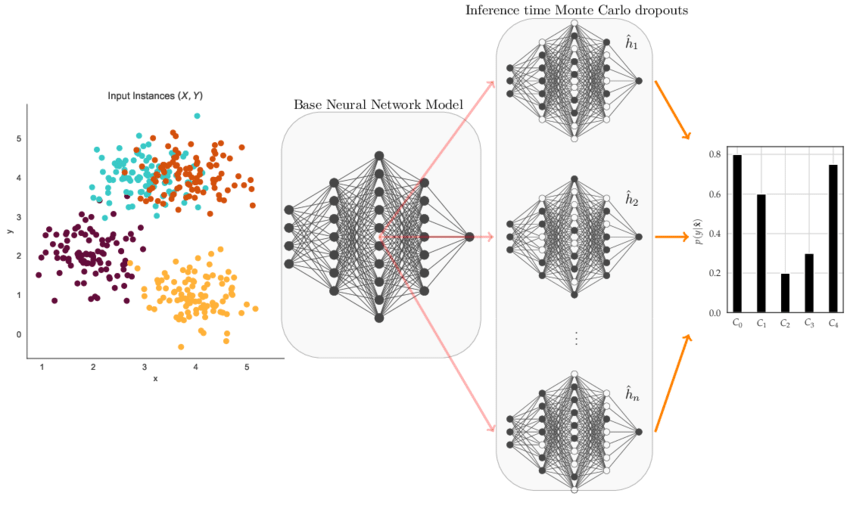
\includegraphics[scale=0.5]{./Images/MCDropout}
	\caption{Monte Carlo Dropout demonstration}
	\label{fig:DNN1}
\end{figure} 
